\documentclass[english,BP]{thesiskiv}

\author{Jakub Matějka}
\declarationmale

\title{Traditional and spiking neural networks}

%
% Texty abstraktů (anglicky, česky)
%
\abstracttexten{Spiking Neural Networks (SNN) are a promising successor to the widely used Artificial Neural Networks (ANN). SNNs aim to be as bio-plausible as possible. However, such behavior is time and energy consuming on the Von-Neumann architecture. Therefore, an entirely new architecture called neuromorphic is being developed and tools to simulate it on standard processors as well. This thesis focuses on comparing the performance of both types of networks in classifying event-related potentials dataset. Two models from each type of network are used and the data are preprocessed in two different ways. The state-of-the-art activation functions, spiking neurons and libraries for simulation are presented. The achieved classification results and the neural models are discussed.}

\abstracttextcz{Impulzní neuronové sítě jsou slibným nástupcem široce používaných tradičních neuronových sítí. Impulzní sítě se drží biologické předloze co nejvěrohodněji. Avšak, takové chování je časově i energeticky náročné na Von-Neumannově architektuře. Proto je vyvíjena zcela nová architektura zvaná neuromorfní a také nástroje pro její simulování na standardních procesorech. Tato práce se soustředí na porovnání výkonu obou typů sítí při klasifikování elektroencefalografických dat. Jsou použity dva modely od každého typu sítí a data jsou předzpracovány dvěma odlišnými způsoby. Jsou prezentovány nejlepší dostupné aktivační funkce, impulzní neurony a knihovny pro simulaci. Dosažené výsledky klasifikací a neuronové modely jsou rozebrány.}


% Na titulní stranu a do textu prohlášení se automaticky vkládá
% aktuální rok, resp. datum. Můžete je změnit:
%\titlepageyear{2016}
%\declarationdate{1. března 2016}

% Ve zvláštních případech je možné ovlivnit i ostatní texty:
%
%\university{Západočeská univerzita v Plzni}
%\faculty{Fakulta aplikovaných věd}
%\department{Katedra informatiky a výpočetní techniky}
%\subject{Bakalářská práce}
%\titlepagetown{Plzeň}
%\declarationtown{Plzni}

%%%%%%%%%%%%%%%%%%%%%%%%%%%%%%%%%%%%%%%%%%%%%%%%%%%%%%%%%%
%
% DODATEČNÉ BALÍČKY PRO SAZBU
% Jejich užívání či neužívání záleží na libovůli autora
% práce
%
%%%%%%%%%%%%%%%%%%%%%%%%%%%%%%%%%%%%%%%%%%%%%%%%%%%%%%%%%%

% Zařadit literaturu do obsahu
\usepackage[nottoc,notlot,notlof]{tocbibind}

% Umožňuje vkládání obrázků
\usepackage[pdftex]{graphicx}

% Odkazy v PDF jsou aktivní; navíc se automaticky vkládá
% balíček 'url', který umožňuje např. dělení slov
% uvnitř URL
\usepackage{url}
\usepackage{breakurl}
\usepackage[pdftex,breaklinks]{hyperref}
\hypersetup{colorlinks=true,
  unicode=true,
  linkcolor=black,
  citecolor=black,
  urlcolor=black,
  bookmarksopen=true}

% Při používání citačního stylu csplainnatkiv
% (odvozen z csplainnat, http://repo.or.cz/w/csplainnat.git)
% lze snadno modifikovat vzhled citací v textu
\usepackage[numbers,sort&compress]{natbib}

\usepackage{amsmath}

% my packages

\usepackage{pdfpages}
\usepackage{listings}

\graphicspath{{img/}}

\def\UrlBreaks{\do\/\do-}
%\interfootnotelinepenalty=10000

%%%%%%%%%%%%%%%%%%%%%%%%%%%%%%%%%%%%%%%%%%%%%%%%%%%%%%%%%%
%
% VLASTNÍ TEXT PRÁCE
%
%%%%%%%%%%%%%%%%%%%%%%%%%%%%%%%%%%%%%%%%%%%%%%%%%%%%%%%%%%
\begin{document}
%
\maketitle
\tableofcontents

% Introduction
\chapter*{Introduction}

Since the beginning of computers people imagined how artificial intelligence (AI) will either help us with everyday struggles, or take over the world one day and destroy us. Today, it is becoming a part of our everyday life, without us even knowing sometimes. We have multiple fields of AI science like expert systems, simple machine learning or advanced neural networks (NN).

A neural networks experience nowadays great development for another time in history. Thanks to stronger hardware and bigger computational capabilities, deep learning became feasible. With this achievement, we are finally able to use NN for purposes in real world. NNs help with predicting diseases, driving cars and they can become fast learners in playing video games.

First part of the thesis researches and examines field of Artificial Neural Networks (ANN) and Spiking Neural Networks (SNN). Current state of neural components like neurons and synapses, algorithms for learning and toolkits will be described. Some advantages and disadvantages will be compared together with differences between ANNs and SNNs.

Goal of this work is to design both ANN and SNN that will classify electroencephalography (EEG) data. Both approaches will be tested and compared according to their accuracy. Data were acquired from people, who were told to think about a number and then their brainwaves were recorded. This work will find out results of different classification approaches with both ANNs and SNNs.

In chapter 1 there is thorough description of both network models with its components. Chapter 2 focuses on training of each network with both supervised and unsupervised learning. Chapter 3 goes over simulation tools for designing both types of networks, including those used for experiment. Chapter 4 introduces neuromorphic hardware including a new component in electronics called memristor. Chapter 5 and following are dedicated to the experiment and results, which are final goal of this work.



% Overview ANN and SNN
\chapter{Overview of artificial and spiking neural networks}
\label{ch:overview}

Neural network (NN) is in its core a complex mathematical function, which models and simulates behavior of brain. Brain contains mainly biological neurons and synapses. In the algorithm of NNs both neurons (Section~\ref{sec:ann_neurons}) and their connections called synapses are mathematical functions.

Each NN has input neurons and output neurons. Those neurons are connected with synapses. The data given to input neurons are processed by the NN and result is received by output neurons. The data is transformed through the NN accordingly to its structure -- type of neurons and synapses, and strength of synapses. Spiking Neural Networks (SNN) use different way to transfer signal than Artificial Neural Networks (ANN). Approaches with differences are described later in (Section~\ref{sec:artificial_nn} and Section~\ref{sec:spiking_nn}).

Nowadays, it is typical for a NN to have more layers of neurons, meaning there is so called hidden layer, or layers of neurons between input and output layer. These are called Deep Neural Networks (DNN). DNNs proved to be more powerful than single-layered NNs, due to possibility to train more layers.

Next part will cover basic properties and differences between artificial and spiking NNs. Main focus is given to differences between these two types of networks.

%
% ARTIFICIAL NNs
%

\section{Artificial neural networks (ANN)}
\label{sec:artificial_nn}

ANNs compute with numerical values. Layers are represented by vectors, matrices or even tensors. It depends on how many dimension does the input layer has. The values are real numbers. With numbers we can apply backpropagation and use an activation functions (Section~\ref{sec:activation_functions}), in order to train an ANNs.

As data travel through the NN, each neuron in ANN uses an activation function in order to decide, whether it will be activated or not. If the neuron is not activated it does not fire further to next neurons.

ANNs are nowadays capable of creating and modifying images, detecting elements in them, or even creating videos from images. Another example of usage are agents (self-controlling models in an unknown environment). We make ANNs drive cars or play games like Chess and Go. First neural network that had beaten human champion in game of Go is named AlphaGo. Researches from other areas took algorithm of AlphaGo and created AlphaZero to play Chess and AlphaStar to play StarCraft.

%
% SPIKING NNs
%

\section{Spiking neural networks (SNN)}
\label{sec:spiking_nn}

On contrary to ANNs, SNNs do not use numbers, but spike trains, which are events increasing potential of neuron's membrane. When the membrane is excited enough, the neuron fires signal forward to all connected neurons. The signals are called spikes and they are pieces of information traveling through network. Membrane potential is then reset after firing. We are able to observe single neuron spikes and tell during which activities neurons are most active.

Due to the fact that SNNs are brain inspired networks, they are built using differential equations. The equations represents membrane and determine frequency of spikes. \cite{snns-nextgen} Calculating differential equations is difficult task for processors with traditional Von Neumann architecture -- it leads to overheating, long computing and high power usage. New architecture for neuromophic computing (computing using SNNs) could provide a solution. For this problem, neuromorphic chips are being built especially for SNNs. With such hardware, SNNs will overcome problems ANNs have on the state-of-the-art hardware, because of better compatibility and smaller energy consumption. Neuromorphic hardware uses both computing and memory unit represented by one piece called memristor. (Section~\ref{sec:memristor})

It is known, that ANNs are hard to interpret and they tend to behave like black boxes. They are usually fully connected (every neuron in one layer is connected to each neuron in following layer) and use vector based computation. Thus have a fixed structure. Brain is built to behave dynamically, in order to adapt quickly. With dynamic networks we would be able to understand their behaviour better. For goal of better interpretability are SNNs better. \cite{neucube}

Several studies show possibility of decoding brain signals from electroencephalography (EEG) during body movements. SNN is able to map encoded EEG signals to 3D reservoir of NeuCube framework and evolve in order to predict brain spikes better. Improved discovery of brain centers with this approach of brain signal decoding and mapping it to NeuCube is promised. \cite{neucube}

This could be helpful for more precise usage of prosthetics after limb loss. Current prosthetics might fulfill their purpose, but they will not simulate human limb perfectly . For new brain inspired brain-computer interface it should be easy task thanks to SNNs' ability to precise spike timing with spike time-dependent plasticity (Section~\ref{sec:unsupervised_snn}) rules. \cite{stdp-biological}

Training SNNs with small dataset gives good results. Human brain has enormous learning capacity and has ability to perform complex task with small energy output, so brain inspired SNNs have the potential to perform better than ANNs. SNNs are called third generation of NNs and thanks to their brain-like structure both training and final use should be faster. Output spikes in the beginning tend to be not precise, but when SNNs are given time to process spikes, they can improve classification abilities. \cite{stdp-biological}

%
% ARTIFICIAL NEURONS
%

\section{Artificial neurons}
\label{sec:ann_neurons}

Neuron is one of the main parts of neural network. In neurons it is decided if signal will continue or not. Each neuron has some amount of input and output synapses, where signals to transfer are coming and leaving.

The simplest type of neuron is perceptron, which was also the very first one made. Single layered perceptron can be used only for linear regression. Later researchers used perceptrons in layers and developed multi layered perceptrons (MLP). With combination of more complex neurons and better activation functions, MLPs are used as good classifiers capable of finding multiple classes, not just two. For example simple classification of pictures with animals.

We can describe perceptron neuron mentioned above with this function:

$$
	y = f(\sum_i{w_i \cdot x_i}) + b
$$

Where $y$ is the final result, which will leave from neuron, $f$ is chosen activation function (Section~\ref{sec:activation_functions}), $w$ is weight of incoming signal and $x$ is input value, which it carries. At last, $b$ is bias, which can help to activate the neuron. The neuron then fires forward or is regressed and stops the signal from going onward.

%
% SPIKING NEURONS
%

\section{Spiking neurons}
\label{sec:snn_neurons}

Various models of spiking neurons is an analogy to activation functions (Section~\ref{sec:activation_functions}) in ANNs. There are new types being developed and every model has its pros and cons. Spiking neurons are created with capacitors and resistors, that simulate bio-chemical reactions of potassium and sodium in brain.


\subsection{Leaky integrate-and-fire (LIF)}%
\label{sub:lif}

LIF is the simplest spiking neuron in terms of bio-plausibility. However, its computational cost is the smallest. Thanks to the low cost, it is possible to simulate large networks with thousands of neurons at once. \cite{brainmodels-lif} LIF is very focused on precisely-timed events carrying the information,  because it is capable of a few spiking shapes. \cite{bisnn-for-decoding-muscle-act}

Functionality is only about accumulating energy until the membrane is excited enough and the energy is released -- fired. Nowadays, LIF is the most used spiking neuron model.


\subsection{Izhikevich}%
\label{sub:izhi}

Izhikevich neuron combines simplicity of LIF neuron (Section~\ref{sub:lif}) and bio-plausibility of Hodgkin-Huxley model (Section~\ref{sub:hodhux}). This makes it more energy consuming, than LIF neuron, but still less than Hodgkin-Huxley. It is capable of various spike shapes, so it makes it a good compromise. \cite{brainmodels-izhi}

Functionality is more complex than the one of LIF neuron, but this model is also accumulating energy and then fires. In addition there is decaying variable, which is put to high value, when Izhikevich neuron fires and then the variable slowly decays (looses its value).


\subsection{Hodgkin-Huxley}%
\label{sub:hodhux}

This neuron model is considered the most bio-plausible, which also makes it very computation demanding. \cite{brainmodels-hh} Hodgkin-Huxley neuron has three channels that together represent functionality of real human neuron. Two channels simulate sodium and potassium bio-chemical reactions. Last channel maintains potential of the neuron and cooperates with other channels while they are closed. \cite{hh-bio-form}

Hodgkin-Huxley neuron received Nobel Prize in Psychology or Medicine in year 1963. \cite{hh-nobel}


\subsection{Legendre Memory Unit (LMU)}%
\label{sub:lmu}

Legendre Memory Unit is new type of spiking recurrent neuron. They already proved to have better accuracy, than standard Long short-term memory (LSTM) neurons when classifying Permuted Sequential MNIST dataset. The LMU consists of layers, where each layer contains nonlinear hidden state and linear memory cell. Hidden state is generated after input to the layer. Important part of the LMU is sliding window, which helps with orthogonalization of time vectors from its input signal. \cite{lmu-article}

%
% ACTIVATION FUNCTIONS
%

\section{Activation functions}%
\label{sec:activation_functions}

Activation function in neuron is used to process the signal that came in. Incoming signal is value going over some synapse multiplied by weight of the synapse. Result is combined with previously mentioned bias value. Next part will describe a few basic activation functions for ANNs.


\subsection{Sigmoid}%
\label{sub:sigmoid}

Sigmoid function is used for normalizing input value to range from 0 to 1. They had been used in deep layers of NNs before discovery of a function Rectified Linear Unit (Section~\ref{sub:relu}), a more advanced function described below.

Mathematical notation of Sigmoid function:

$$%
	f(x) = \frac{1}{1+e^{-x}}%
$$


\subsection{Rectified Linear Unit (ReLU)}%
\label{sub:relu}

ReLU transforms all negative values to zero and other values leaves untouched. That means it is easy for computation and is able to converge to minimum faster. With ReLU we can train NNs faster with higher accuracy. However, disadvantage of this function is that neurons tend to die often as a consequence of the negative numbers transformation to zero.

Mathematical formula of ReLU function is

$$%
	f(x) = \begin{cases} 0 & \text{if } x < 0 \\
						 x & \text{if } x \geq 0.%
			\end{cases}%
$$


\subsection{Swish/SiLU}%
\label{sub:swish_silu}

Swish function was introduced after ReLU function. Negative numbers are not changed to zero, but kept as a small negative value. It can perform better than ReLU, but it is computationally more demanding. \cite{swish}

The $\beta$ in the equation is either constant or trainable parameter. First version of Swish function is without the $\beta$. It was added there later, when the second version of paper \cite{swish} was released.

Mathematical notation of Swish function is

$$%
	f(x) = x \cdot \text{sigmoid}(\beta x).%
$$

Independently, there was discovered same function, but named Sigmoid-Weighted Linear Unit (SiLU). \cite{silu} An object of this function is in the Tensorflow library (Section~\ref{sub:tensorflow}) created with \texttt{tensorflow.nn.silu}. Although, in Keras \ref{ssub:keras} can be found as \texttt{tensorflow.keras.activations.swish}.


\subsection{Softmax}%
\label{sub:softmax}

Softmax function is usually applied in last layer of NN. It is probabilistic function, that can distribute values in a way that their sum is equal to one. Thus we can determine probability of various classes, which the NN have to classify.

Mathematical notation of Softmax function is

$$%
	f(x) = \frac{e^{x_i}}{\sum\limits_{j=1}^{n} e^{x_j}} \quad \text{for } i=1,2,\dots n.%
$$



% Training of SNNs
\chapter{Training of neural networks}%
\label{cha:training_nns}

Training of ANNs is nowadays very developed and there are many algorithms for various tasks. Advantage is computing with real numbers and lesser complexity of mathematical equations. Von Neumann architecture is quite well suited for this purpose, although it still suffers from slow byte exchange between CPU and RAM.

On the other hand, training of SNNs is still a challenge due to their non-differential nature and other reasons like non-native hardware, inability to use well known and mainstream training algorithms or even absence of proper programming language for an essence of SNNs and neuromorphic hardware (Section~\ref{cha:neurom_hw}). Not only that efficient training algorithms are missing, but they are hard to design, due to asynchronous calculations. \cite{dl-with-sneurons}

Researchers are coming up with new ways how to improve usability of SNNs. Results so far suggest that SNNs might be stronger in given tasks than ANNs in the future. \cite{dl-in-snns}

For accurate SNN it is important to have precise timing of spikes and firing patterns, if we want them to simulate brain very well. To achieve this we need to pick well designed and programmed synapses, neurons and use complex datasets for benchmarking. It is important, because even small difference or single spike can produce different behaviour. \cite{dl-with-sneurons}

In brain, there are excitatory and inhibitory neurons, which cooperate together, in order to keep brain function properly. SNNs use similar approach, but with synapses, for giving accurate results. Excitatory synapses increase potential of neuron's membrane and inhibitory decreases it. This ability is important part of training, but remains a challenge for current learning methods, because we cannot use back-propagation algorithm. Solution came with spike time-dependent plasticity (STDP), which is set of learning rules. STDP is described in Section~\ref{sec:unsupervised_snn}.

Deep learning in SNNs usually uses only one learning layer and one layer for classification. In the beginning of deep SNN are a few layers for preprocessing. Whereas for ANNs there are many options how to put layers together. Network with dense layers is fully connected and last layer is for classification. Convolutional network take turns of convolutional and max-pooling layers and in the end there are dense layers. Recurrent networks have some layers in cycles.


\section{Unsupervised learning of ANNs}%
\label{sec:unsupervised_ann}

We use unsupervised learning for unlabeled datasets. This is useful for association, clustering and finding patterns or anomalies in data. NNs trained unsupervised way are able to draw images, write stories or compose music. Nevertheless final pieces are not the best and there is still a lot to be improved.

NN has to learn on its own similarly like children are learning. It processes given data and then adjusts its weight and biases, in order to minimize the error -- difference between given input and final result. After training the network should be able to give similar samples like in dataset, even if it is given noise samples.

During this approach it is common to use competitive learning rules like winner-take-all.


\section{Supervised learning of ANNs}%
\label{sec:supervised_ann}

Supervised learning can be used with labeled dataset. We know what every sample is and what it means. Then we can give it to ANN to process and compare its results with desired label. It means that an input vector of data is compared with an output vector. If the result is wrong, then the error is backpropagated to the network with loss function a gradient descent algorithms, that corrects network's weight and biases.

Due to the fact, that we have labeled data, one problem may arise, and it is overfitting. Overfitting happens, when NN is trained too much and thinks it will receive only samples like it had in training dataset. NN will classify new unseen samples as classes it encountered during training, even though the samples belong to different class, but they are very similar.

Supervised learning is good for classification tasks -- we have two or multiple classes and we want the network to identify, which class a sample belongs to. And regression tasks -- we have data and we want to predict how they will develop.


\section{Unsupervised learning of SNNs}%
\label{sec:unsupervised_snn}

Unsupervised learning of SNNs reminds us of real brain function. Main used set of unsupervised learning is spike time-dependent plasticity (STDP). SNNs learns by adjusting weights of pre- and post-synaptic neurons, in order to improve spike times. Meaning, the weight of synapse between neurons is strengthened, when pre-synaptic neuron fires before post-synaptic neuron. The strengthening is called long-term potentiation (LTP). And the weight is weakened, when pre-synaptic neuron fires after post-synaptic one. The weakening is called long-term depression (LTD). This means that neural path are created with high information flow on path from beginning to end of network. With STDP rules, even single neuron is able to recognize and learn repeating patterns of spikes. \cite{dl-with-sneurons}

STDP has potential to be very bio-plausible, because it is inspired by real processes in brain \cite{stdp-biological}. However, with higher bio-plausibility comes high complexity in computations and hardware implementation. STDP is also good for sequential data processing \cite{survey-stdp}, so EEG data decoding application with this learning is in situ.


\section{Supervised learning of SNNs}%
\label{sec:supervised_snn}

Supervised learning of SNNs, on the other hand, is similar to backpropagation used in ANNs, like gradient descent. Here we want to get as close value of output spike to desired one as possible and minimize the error. From this point researches could start developing gradient descents for SNNs. \cite{backprop-snns}

For gradient descent we need real values and not spikes. Best real values found in SNN are those of membrane's potential. A deep SNN is capable to train from spike signal patters and reach state-of-the-art results. \cite{dl-with-sneurons}


\section{Transformation ANN to SNN}%
\label{sec:trans_ann2snn}

Classic way to train a neural network is unsupervised or supervised learning. Nevertheless, there are also experiments with converting a trained ANN to SNN. This SNN development give plausible results in many cases. \cite{dl-in-snns}
To achieve conversion, ANN is trained with standard algorithms first, and then artificial neurons are changed to spiking neurons. Conversion works for fully connected networks, convolutional networks, deep belief networks and recurrent networks too.

Recurrent neural networks (RNN) are great for one-dimensional and sequential data, so it is great candidate for EEG data processing. The best model of recurrent networks is the long short-term memory (LSTM). Specifically, this set of models is called gated recurrent networks (GRU). The models are called gated, because the consist of cells with gates controlled by trainable weights. It makes sense to start converting RNNs first and test them as spiking RNNs.

Although not every ANN can be easily converted to SNN. Values of spiking neurons are always positive. This is a problem when there is a conversion of neuron with negative activation. As mentioned in Section~\ref{sec:artificial_nn}, artificial neurons use real numbers, including negative ones. Solution could be ReLU activation function (Section~\ref{sub:relu}) with its outputs being either zero or positive values. With such values it will be easy to convert neurons. Another improvement is to create two spiking neurons from an artificial neuron, and let one handle positive values and the other one negative values. \cite{2ann-for-1snn-neuron}

Of course if we wanted to convert network super precisely, it would be at cost of more spiking events and more energy consumption.



% Simulation toolkits
\chapter{Simulation tools}
\label{ch:simulation_tools}

This chapter describes tools for designing ANNs and simulating SNNs. Neuromorphic hardware is still not available for wide population, so we are using simulators of such hardware. Included simulators are those highly used and actively developed.

%
% Traditional neural networks tools
%

\section{Traditional neural networks tools}%
\label{sec:traditional_neural_networks_tools}

At first we will look at tools for ANNs. Presented are two most used -- Tensorflow and PyTorch. But there are also other libraries such as Aesara, fork of Theano (Theano is not being developed anymore), or Keras, which is high-level library with API for Tensorflow and Theano as a backend.


\subsection{Tensorflow}%
\label{sub:tensorflow}

Tensorflow is a library for machine learning (ML) developed by Google Brain Team. It is written in C\verb!++! with Python high-level API, with CUDA support, and released under Apache License 2.0. First version of Tensorflow focused on building static graph, which represents ANN, before execution. This approach is good for debugging purposes and the graph analysis, but it does not allow developer to change the graph during runtime. Version two of Tensorflow was inspired by PyTorch (Section~\ref{sub:pytorch}) and started using objects. Like this it is easier to design various layers of ANN and it is possible to change them during runtime.

Tensorflow provides tool Tensorboard, where developers can analyze ANN in depth and see exact results. \cite{tensorflow}


\subsubsection{Keras}
\label{ssub:keras}

Keras is high-level API for ML libraries developed by a Google engineer François Chollet. It requires proper library as a backend and provides easy programmable interface. Developers are able to avoid usage of backend ML library itself, which can be sometimes complicated.

At first, it was developed independently of Tensorflow and provided multiple backends like Theano or CNTK, but from Keras version 2.4 only Tensorflow is supported. Tensorflow served as a main backend since Keras version 1.1 already. Nowadays Keras is included in Tensorflow in submodule \texttt{tensorflow.keras} and should be used from there. Standalone Keras library is receiving only bug fixes. \cite{keras}


\subsection{PyTorch}%
\label{sub:pytorch}

PyTorch is developed by Facebook AI Research lab (FAIR). Like Tensorflow, it is written in C++ with Python API, with CUDA support, but released under BSD-style license. It provides tensor computation with GPU acceleration. \cite{pytorch}

As said before, PyTorch allows developer to create neural models as classes with defined layers as class attributes. That gives us a free hand to design models as we want. PyTorch also works well with Matplotlib, NumPy or SciPy library. PyTorch has implementation focused on performance, due to some Python's limitations. Besides efficient C++ core, it separates control and data flow, meaning that basic program flow, like branches and loops, are executed on CPU, whereas tensor operations are executed on GPU. If given computer has CUDA enabled GPU, of course. Another performance improvements are incremental memory allocation on GPU with CUDA, and object reference counting, that allows PyTorch to smartly deallocate no longer needed tensors. \cite{pytorch-paper}

%
% Spiking neural networks tools
%

\section{Spiking neural networks tools}%
\label{sec:spiking_neural_networks_tools}

ANN toolkits receive a lot of attention from the public, but SNN toolkits are better known among researchers. Tools for SNNs simulations are introduced in this section.


\subsection{Nengo}%
\label{sub:nengo}

Nengo is a framework for designing large scale networks. Version 1 was written in Java, but version 2 is rewritten in Python from scratch for higher speed. Currently it is the fastest running solution for creating networks with hundreds and more neurons. \cite{nengo} It is built on a theoretical framework called the Neural Engineering Framework (NEF), which is designed for large scale approach of network modeling. NEF proposes three principles allowing to model large scale networks. The three principles are Representation, Transformation and Dynamics.

For Representation Nengo provides \textsf{Ensemble} object. It is population of neurons represented by time-varying vector with real numbers allowing us to encode it and decode it.

For Transformation Nengo provides \textsf{Connection} object. It allows us to create synapses among populations of neurons and connect them, so the neurons can communicate among each other.

Dynamics principle is created, when \textsf{Ensemble} object is connected to itself. Like this we can create recurrent parts of our networks.

Nengo also provides another objects like \textsf{Node} for accepting input and processing output from it, \textsf{Probe} for collecting data during a simulation, and \textsf{Network}, which represents whole designed network composed from available objects.

Nengo is available for non-commercial use released under proprietary license.


\subsubsection{NengoDL}
\label{ssub:nengodl}

NengoDL (Nengo Deep Learning) is a branch of Nengo created to make Tensorflow (Subsection~\ref{sub:tensorflow}) components and models compatible with those in Nengo. NengoDL provides \texttt{nengo\_dl.Converter} for easy and almost automatic Tensorflow neural model conversion to Nengo model. However, it is also possible to convert single model components (like layers and activation functions (Section~\ref{sec:activation_functions})) manually with more specific methods in NengoDL. Currently it is the easiest solution to transform ANN model to SNN model.


\subsection{Brian2}%
\label{sub:brian2}

Brian2 is framework written in Python, that aims to be easy to use for mathematical scientists. Models are written in mathematical form; similarity as equations. Brian2 is also able to generate code in background, due to its high-level scripting. Generated code is inserted into working piece of code, thanks to the framework. \cite{brian}

There is a number \textit{2} in the name, because it was rewritten, in order to improve speed. First version of Brian is now legacy code. Brian2 uses vectorized algorithms in core \cite{brian-vectorized}, which makes it faster than NEST simulation tool (Section~\ref{sub:the_network_simulation_tool_nest}) for homogeneous neuron population. For heterogeneous population, their speeds are comparable. \cite{brian}

Writing plugins for this framework is possible. For example Brian2GeNN \cite{brian2genn} for GPU computation support or Brian2CUDA \cite{brian2cuda} for CUDA parallel support. GPU acceleration is able to increase speed by tens to hundreds of time.

Brian2 is released under CeCILL 2.1 license.


\subsection{The Network Simulation Tool (NEST)}%
\label{sub:the_network_simulation_tool_nest}

NEST is built for dynamics, size and structure of neural systems, giving researches ability to shape models to their needs. NEST provides over 50 neuron models and over 10 synapse models, which gives the toolkit lots of flexibility, as well as the fact that multiple neurons and synapses can coexist together. NEST was developed in 1994 and is expanding and improving since then. NEST itself is simulation program with core written in C++ and PyNEST allows us to control it with Python. \cite{nest-site, nest}

NEST is one of many services offered by EBRAINS, which is a digital research infrastructure providing state-of-the-art capabilities for collaborative brain research. \cite{ebrains} EBRAINS is powered by Human Brain Project (HBP) \cite{hbp}. HBP is building research infrastructure across Europe, in order to completely discover and understand complexity of human brain.

NEST is released under GPL-2.0 license.



% Neuromorphic hardware
\chapter{Neuromorphic hardware}%
\label{cha:neurom_hw}

As mentioned before in Section~\ref{sec:spiking_nn}, neuromorphic hardware (NMHW) is becoming new computing architecture specifically designed for SNNs. Current computer architecture -- Von Neumann architecture, is sufficient for computing, but there is still overhead due to separated computing unit and memory unit. Data needs to be transferred from memory to computing unit over bus. That costs time and energy on this architecture for simulating algorithms as SNNs.

Although spikes are sparse in time, one spike train carries high information amount. Thanks to this we will be able to design low energy consumption hardware. SNNs should be run on NMHW, because of easier information propagation, power efficiency and in-memory computing. All units in Von Neumann architecture work synchronously driven by internal clock. Both NMHW and neurons in SNNs are not synchronized by clock, but actions inside happen in parallel, which leads to great asynchronous computing. NN model using sparse temporal codes should benefit more from NMHW, because energy is taken by synaptic events the most. \cite{dl-with-sneurons}

Real NMHW called TrueNorth, SpiNNaker and BrainScaleS with silicon chips already exists. Their production is costly and time-consuming, so they are not for sale yet. NMHW is not available for general public, however, there are cloud data centers being built, with access to SpiNNaker and BrainScaleS systems. \cite{ebrains}

The EBRAINS offers free and quick access to brain inspired computing devices for researchers. Certain thing is also API opened for Python scripts.
Intel company also develops neuromorphic chip called Loihi and gives access to limited amount of the chips for researching. Loihi possesses big amount of interconnected neurons, low power consumption, self-learning and on-chip learning. \cite{intel}

Besides cloud computing, NMHW is good candidate for embedded devices like battery-powered robots, mobile phones and internet-of-things devices.

\section{Memristor}%
\label{sec:memristor}

Memristor is a memory resistive device developed by HP labs, which gained popularity in 21st century. Memristors found use for NMHW, after further exploration, because they allow us to avoid the bottleneck of Von Neumann architecture. Synaptic connections of human brain are imitated by memristor. Synapse models act as memory and occupy the biggest area in chips, so its optimization is essential. Complexity of synapses also grows with bio-plausibility and they require more space when implemented in silicon. Memristors are more energy efficient then regular transistors and they show STDP-like (Section~\ref{sec:unsupervised_snn})  behaviour. \cite{fpga-impl-nn}

NMHW technology with memristors was not very well suited for ANNs, because synaptic weights are stored in SRAM or DRAM (static and dynamic random access memory) and these hardware components are too big to be implemented in high amount. However, after many improvements of memristors, it is now possible to implement ANNs on NMHW better. On the other hand, NMHW with memristors is very well suited for SNNs. It takes lots of computation to simulate SNNs on Von Neumann architecture. SNN is implemented with CMOS and memristors. The former works as neurons and the latter as synapses. They are combined together in a grid and can work both as memory and computational unit, so Von Neumann bottleneck is removed. Applicability of these components is both space and energy efficient. Also, SNNs does not need to calculate everything at once, in contrast to ANNs, which calculate layer by layer. SNNs spread its computation, so those neurons, that does not receive any input, can go to standby mode. In the end the energy consumption is lower. ANNs still remain target to be implemented and experimented with, but SNNs promise great potential in this area. \cite{memristors}



% Experiment
\chapter{Experiment}%
\label{cha:experiment}

Now, when important theoretical concerns are discussed we will move to experiment with NNs on EEG brain data. This chapter will describe used dataset and methods with NN models during experiment. Achieved results are presented as last part and later discussed.

This experiment was based on paper \cite{varekap300}. The aim was to classify retrieved brainwave data to classes of target and non-target numbers (meaning explained in Section~\ref{sec:dataset}) with supervised learning of NNs. (Section~\ref{sec:supervised_ann}, Section~\ref{sec:supervised_snn}) In the original paper, author was able to achieve accuracy of 62-64\% when classifying single-trial components (one 1200 ms long stimuli sample), but when averaging of the components was applied, the accuracy increased to 76-79\%. The author main used NN model was 2D Convolutional ANN.

Classification with both ANNs and SNNs, together with both single-trial data and data averaging, was the goal during this experiment

%
% DATASET
%

\section{Dataset}%
\label{sec:dataset}

Dataset consists of P300 brainwaves retrieved from 250 school-age children (138 males and 112 females). Authors of the dataset visited elementary and secondary schools and let children participate in an experiment. The children were asked to choose a number in a range of 1 to 9 during the experiment. The chosen number is referred to as the \textit{target} number and other numbers are referred to as the \textit{non-target} numbers. After a participant's choice, they were show a random number for one second long interval and had to focus, when their number appeared. Their brain waves were recorded from three channels (Fz, Cz, Pz) in total, 200 ms before start of the stimuli and 1000 ms during it. The result is 1200 ms long sample in three vectors for one stimulation. Total amount of samples is 11~532. Participants were stimulated with multiple numbers within a few minutes.

How dataset was processed during the experiment is described in a following section. Dataset is available at \cite{dataset} and thoroughly described in \cite{dataset-article}.

%
% METHODS
%

\section{Methods}%
\label{sec:methods}

For the experiment, Tensorflow (Subsection~\ref{sub:tensorflow}) and NengoDL (Subsection~\ref{ssub:nengodl}) were used, due to their good compatibility. Both libraries were used with their Python API. Models were trained and tested on CPU Intel~i5-8300H. Following part describes used pre-processing, neural models and how training was done.

%
% PREPROCESSING & TRAINING
%

\subsection{Pre-processing and training}%
\label{ssec:preproc_train}

The dataset \cite{dataset} can be loaded as a Python dictionary. It is divided into two parts -- part with target numbers under key \texttt{allTargetData} and part with non-target numbers under key \texttt{allNonTargetData}. The data were filtered to remove damaged samples for example after blinking or distractions from surroundings. A threshold for the filtering was set to $100\ \mu V$ from both sides, so all signals with higher value than $100\ \mu V$ or lower than $-100\ \mu V$ were removed. The~samples were labeled afterwards with hot-encoded vector (1,~0) for targets and vector (0,~1) for non-targets. The~signals from all three channels were joined together into one vector with length 3600 (3~$\times$~1200~recorded milliseconds) creating one long signal. Then the matrices of targets and non-targets were concatenated together with their labels, which created a matrix of size $8036 \times 1 \times 3600$ (number of samples $\times$ channels $\times$ number of features).

Above described is data preparation without averaging. As suggested in original paper \cite{varekap300}, averaging helped to increase accuracy of used Convolutional ANN. The~averaging, which is the aim of this experiment, was approached in two ways here.

\begin{enumerate}
	\item Processing version 1 (PV1) averaged consecutive values in a signal with sliding window of size 3, 6 and 9. The channels for this step had to be preserved (they were joined into the shape described above later). The window was gradually iterating over the values in the signal and was creating new values. Essentially smoothening the signal. Consequence was shortening the signal by the window size minus one. Using values from the beginning of the signal to average them with the values in the end could create unwanted artifacts, that could lower accuracy -- signal would not be continuous. This was done for all three channels and like this new sample for a one person was created.

		When data were in correct form, they were randomly split in ratio 80\% for training data and 20\% for testing data. And during training, the training data were randomly split in ratio 80\% for actual training data and 20\% for validation data.

	\item Processing version 2 (PV2) was averaging whole samples (the reshaped 3600 long vector) among all people randomly. The amount of samples to average here together was 3, 6, 9, 12 and 15. There was a matrix with random values generated for this approach. The height of the matrix was optional and represented amount of new samples in a training dataset part. The width was the averaging amount. In the rows there were indexes of samples from the original dataset to average. Like this it was possible to create entirely new training dataset with optional size. Therefore, training size was set to 10~000 and then to 20~000 samples. The \textit{original dataset} was used as \textit{testing data}. So~the models were trained on artificial generalized data and were tested on untouched data from a real world.
\end{enumerate}

\textit{Cross-validation} was set to 10, meaning there were 10 different model instances of one NN model (all models are described in Subsection~\ref{sub:nn_models}) and the training data were randomly split 10 times for every new model. After training, test data were given to model for prediction and metrics were collected. Final results (Section~\ref{sec:results}) are averages from all cross-validation iterations.

In the beginning of script there is randomness set to zero value, in order to get reproducible results\footnote{Although, network with LSTM layers does not produce same result after rerun. There is an opened issue on GitHub already (June 2021). \url{{https://github.com/tensorflow/tensorflow/issues/18323}}}. All models were trained for 30 \textit{epochs} with \textit{early stopping} set to value of 5. It means that training will stop, if training loss and validation loss function value will not improve for 5 epochs. Train and test \textit{batch size} was set to 32 for PV1 and 50 for PV2. Small change during the second preprocessing was setting the batch size to 100 for model 4 with LMU neurons -- it performed better that way, so final results in Table~\ref{tab:results_samples_10000} and Table~\ref{tab:results_samples_20000} are from training this way. Collected metrics are \textit{accuracy}, \textit{precision}, \textit{recall}, \textit{F1-score} and \textit{confusion matrix}.

%
% NN MODELS
%

\subsection{NN models}%
\label{sub:nn_models}

There were four NN models used in total. Two ANN models and two SNN models. One SNN was converted from ANN model and the other one was created from scratch with novel LMU neurons (Section~\ref{sub:lmu}). ANN models were compiled with \textit{Adam optimizer} and \textit{binary cross-entropy} loss function. Both ANNs used \textit{ReLU} activation function (Subsection~\ref{sub:relu}) in deep layers and \textit{Softmax} function (Subsection~\ref{sub:softmax}) in the output layer.

Difference of the two ANNs is that the first created contained 1D convolutional layer and 1D average pooling layer, while the second one contained two LSTM layers. As mentioned earlier, in the original paper \cite{varekap300} 2D convolutional layers were used, but in this experiment just 1D convolutional layers were used in order to keep one-dimensionality of brain signal and not to convolve different channel signals together. For second ANN were chosen LSTM layers in order to test performance of Recurrent NN as well, because they achieve very good results with processing 1D data. The architecture of the ANNs can be seen in Figure~\ref{fig:arch_anns}. Implementation and detailed parameters of the Convolutional ANN can be seen in Listing~\ref{list:code_ann1} and the LSTM ANN can be seen Listing~\ref{list:code_ann2}. Summary of used models for better orientation can be found in Table~\ref{tab:models}.

\begin{table}[ht!]
	\centering
	\begin{tabular}{c c c c}
		\hline
		Index & Type & Converted & Layers description \\
		\hline
		1 & ANN & no & 1D Convolutional \\
		2 & ANN & no & Long Short-Term Memory \\
		3 & SNN & yes & converted convolutional ANN (index 1) \\
		4 & SNN & no & Legendre Memory Units \\
		\hline
	\end{tabular}
	\caption{Artificial and spiking neuron network models used in the experiment.}
	\label{tab:models}
\end{table}

SNN model index 3 (see Table~\ref{tab:models}) was made by converting the Convolutional ANN (index 1). The~conversion was done with NengoDL (Subsection~\ref{ssub:nengodl}). Nengo offers a good spiking neuron alternative for ReLU activation function -- \texttt{nengo.SpikingRectifiedLinear}. So the ReLUs were swapped with the spiking neuron from Nengo. \textit{Synaptic smoothing} during the conversion was set to 0.01. This is useful for keeping spike values over more timesteps and not just during their one timestep spiking activity. It~helps the network to have more continuous values and it should help to improve performance. \textit{Firing rates scaling} was set to 1000 to make neurons spike more, so they could update output signal more often. It should work well with ReLU, because it is a linear activation function and the scaling applies linear scale to the signal. Nevertheless, it is possible that scaling will not work well with different activation functions. Although NengoDL is capable of conversion convolutional layers and ReLU functions, it cannot convert layers for batch normalization, average pooling and dropout (regularization). NengoDL also cannot automatically convert Softmax function used in output layer of model 1 (see Table~\ref{tab:models}). Nengo has Sigmoid neuron in API (\texttt{nengo.Sigmoid}), but it is non-spiking and firing rate scaling cannot be applied to it, because the activation function does not support amplitude. Thus it does not perform well. When NengoDL encounters some component, which it cannot convert to its native object, then \texttt{nengo\_dl.TensorNode} is used. The \texttt{nengo\_dl.TensorNode} object is capable of inserting Tensorflow (Section~\ref{sub:tensorflow}) code into Nengo model.

The model 3 was created right after model 1 finished training and testing. The model 3 was tested just with NengoDL, because it was already trained. It is possible to create a model in Tensorflow, convert it to NengoDL model and then train it. Regardless, after a few tries and different approaches, the model trained this way was still performing badly, so it is not included. Only the model trained with Tensorflow and later converted to spiking model is kept. The conversion process is displayed in Listing~\ref{list:code_snn1}.

Last model 4 is implemented only with NengoDL and consists of input node, two LMU neurons (Section~\ref{sub:lmu}) and output node. The architecture uses 212 units and 256 memory dimensions as it is in the original paper \cite{lmu-article}. Just the time window changes size according to samples size. Details of model 4 are displayed in Listing~\ref{list:code_snn2}. The version of used LMU neuron can be found here \cite{lmu-nengodl-doc}. This version is implemented for NengoDL, so it contains a \texttt{nengo\_dl.TensorNode} inside, which makes it not possible to use with a pure Nengo, however, there is an implementation for pure Nengo as well \cite{lmu-nengo-doc}.

\begin{figure}[ht!]
	\begin{minipage}{0.5\textwidth}
		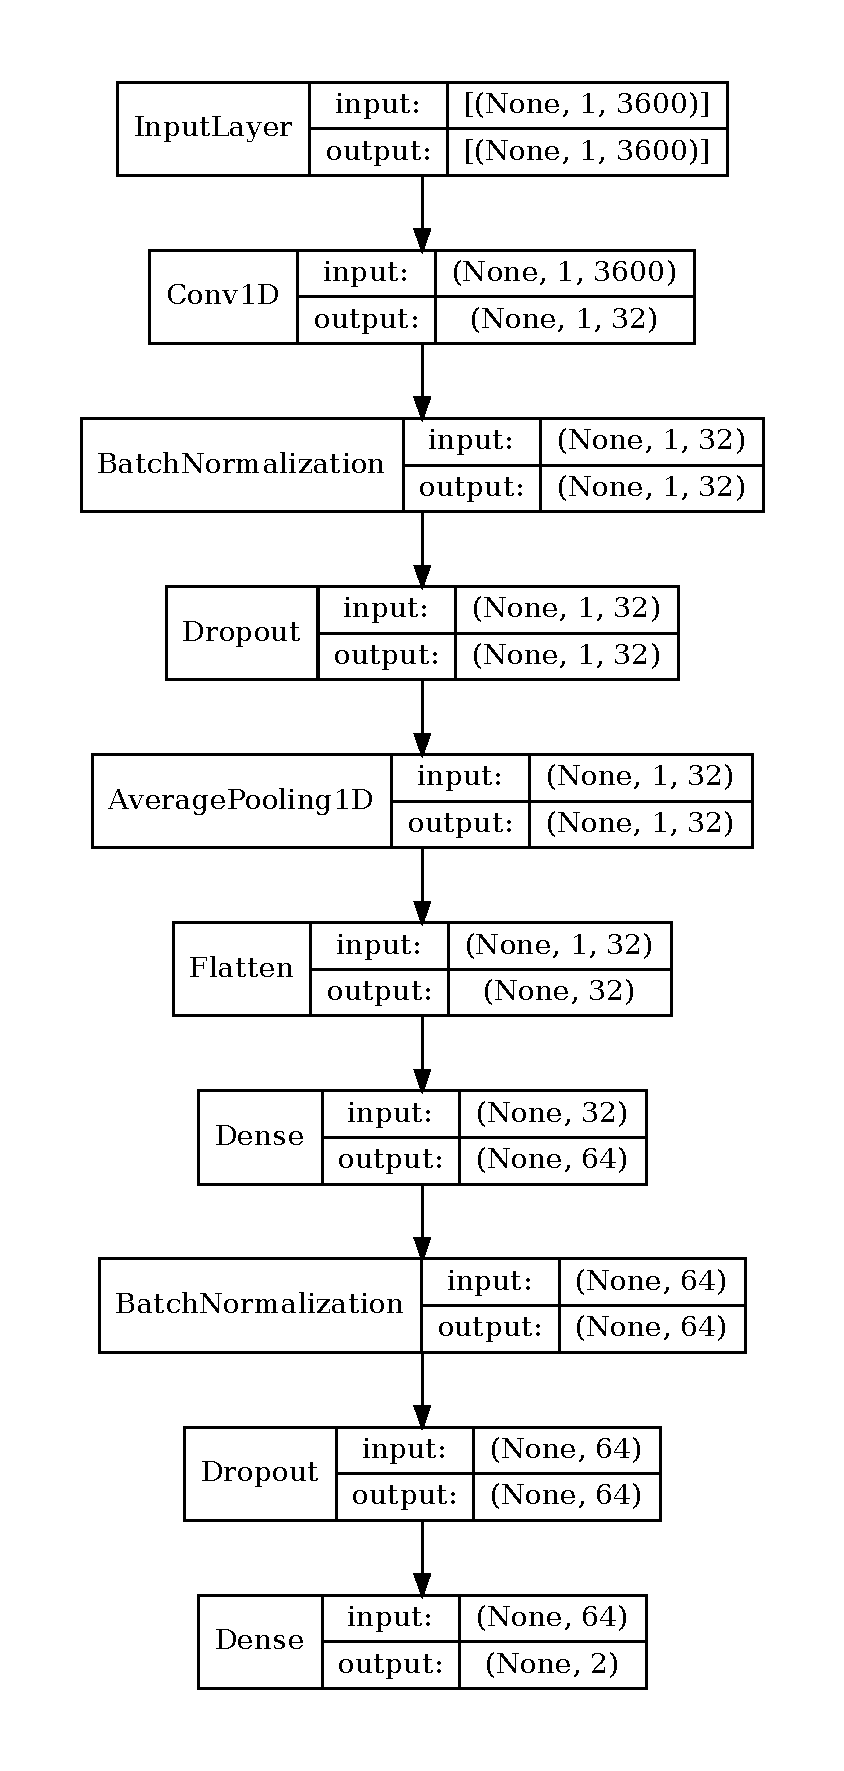
\includegraphics[width=\linewidth]{model_conv.pdf}
	\end{minipage}
	~
	\begin{minipage}{0.5\textwidth}
		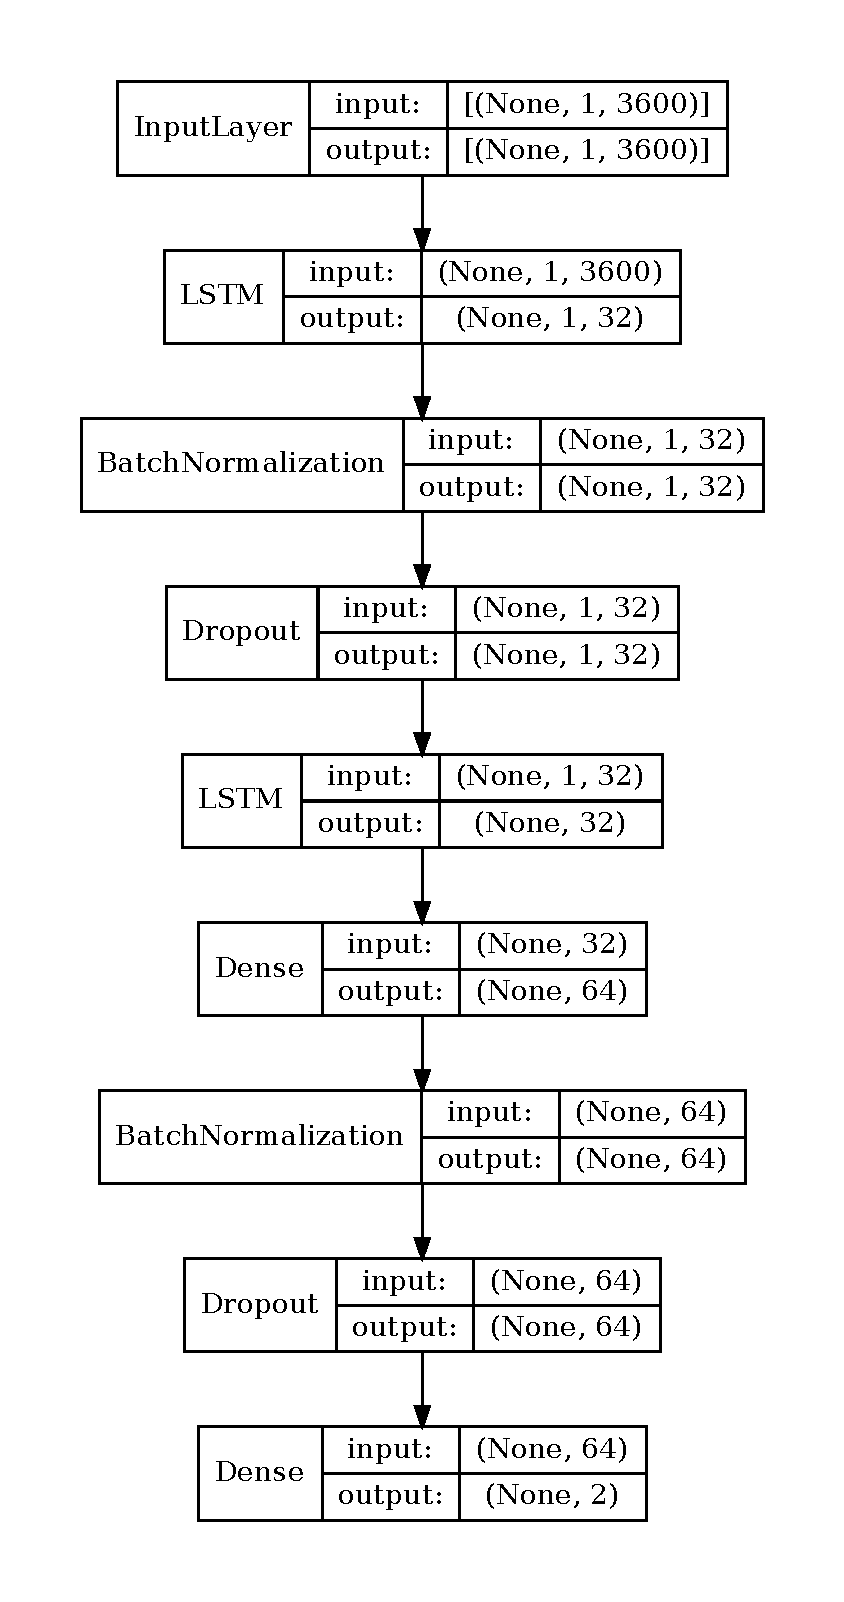
\includegraphics[width=\linewidth]{model_lstm.pdf}
	\end{minipage}
	\caption{Artificial neural networks from experiment. On the left-hand side is the 1D Convolutional ANN and on the right-hand side is the ANN with LSTM layers.}%
	\label{fig:arch_anns}
\end{figure}

\begin{lstlisting}[language=Python,label=list:code_ann1,caption=Implementation of 1D Convolutional ANN.,captionpos=b,frame=single,float]
model = Sequential([
  Conv1D(filters=32, kernel_size=8, strides=4,
    padding='same', activation=relu,
    input_shape=(inp_data.shape[1], inp_data.shape[2])),
  BatchNormalization(),
  Dropout(rate=0.3, seed=SEED),
  AveragePooling1D(
    pool_size=4, strides=1, padding='same'),
  Flatten(),
  Dense(64, activation=relu),
  BatchNormalization(),
  Dropout(rate=0.4, seed=SEED),
  Dense(2, activation=softmax),
])
model.compile(
  optimizer=Adam(learning_rate=0.001),
  loss=BinaryCrossentropy(),
  metrics=['acc', 'mae',
    tf.keras.metrics.Recall(),
    tf.keras.metrics.Precision()]
)
\end{lstlisting}

\begin{lstlisting}[language=Python,label=list:code_ann2,caption=Implementation of Long Short-Term Memory ANN.,captionpos=b,frame=single,float]
model = Sequential([
  LSTM(units=32, activation=relu,
    return_sequences=True),
  BatchNormalization(),
  Dropout(rate=0.3, seed=SEED),
  LSTM(units=32, activation=relu),
  Dense(64, activation=relu),
  BatchNormalization(),
  Dropout(rate=0.4, seed=SEED),
  Dense(2, activation=softmax),
])
model.compile(
  optimizer=Adam(learning_rate=0.001),
  loss=BinaryCrossentropy(),
  metrics=['acc', 'mae',
    tf.keras.metrics.Recall(),
    tf.keras.metrics.Precision()]
)
\end{lstlisting}

\begin{lstlisting}[language=Python,label=list:code_snn1,caption=Conversion of ANN model 1 to SNN model 3.,captionpos=b,frame=single,float]
converter = nengo_dl.Converter(
  model=model,
  swap_activations={
    tf.keras.activations.relu:
      nengo.SpikingRectifiedLinear()
  },
  scale_firing_rates=3000,
  synapse=0.1,
)
\end{lstlisting}

\begin{lstlisting}[language=Python,label=list:code_snn2,caption=SNN model with Legendre Memory Units.,captionpos=b,frame=single,float]
with nengo.Network(seed=SEED) as net:
  # input node for data
  inp = nengo.Node(np.ones(inp_data.shape[-1]))
  # LMU cell
  lmu1 = LMUCell(
    units=212,
    order=256,
    theta=inp_data.shape[-1],
    input_d=inp_data.shape[-1])
  lmu2 = LMUCell(
    units=212,
    order=256,
    theta=inp_data.shape[-1],
    input_d=212)
  # output node for probing result data
  out = nengo.Node(size_in=2)

  # input node is connected with LMU's `x` variable,
  # where input vectors flow into
  nengo.Connection(inp, lmu1.x, synapse=None)

  # LMU's hidden state is kept in a variable `h`
  # it is also an output connected to output node
  nengo.Connection(lmu1.h, lmu2.x,
    transform=nengo_dl.dists.Glorot(), synapse=None)

  nengo.Connection(lmu2.h, out,
    transform=nengo_dl.dists.Glorot(), synapse=None)

  # probe for collecting data
  p = nengo.Probe(target=out)
\end{lstlisting}

\newpage

%
% RESULTS
%

\section{Results}%
\label{sec:results}

Final results of all models with different averaging of \textit{brain signals} (the PV1, see Subsection~\ref{ssec:preproc_train} point 1) can be seen in Table~\ref{tab:results_signals}. Results of all models, that were fed with averaged random samples (the PV2, see Subsection~\ref{ssec:preproc_train} point 2) from artificially created dataset of size 10~000 samples can be seen in Table~\ref{tab:results_samples_10000} and results from models fed with the same way created dataset of size 20~000 are in Table~\ref{tab:results_samples_20000}.

In tables, there is accuracy, precision, recall and F1-score presented from previously mentioned collected metrics. Convolutional models were performing the best with accuracy of 63-64\% after PV1. After PV2, convolutional models were giving the best results again with accuracy of 64-66\%. This~accuracy was achieved with 10~000 artificial samples. But when the sample amount was doubled to 20~000, the accuracy increased to 65-68\%.

The transformed Convolutional ANN to Spiking Convolutional NN was always very close to original model with performance. When it outperformed the original model, it was by very small amount. LSTM network performed worse than 1D Convolutional network. And novel SNN with LMU neurons also did not outperform the convolutional networks. The LMU was actually the worst performing network, which was not expected, since it promises better performance than LSTM and since it is a spiking network, so it should handle one-dimensional input very well.

Generally PV1 did not have noticeable effect on the networks. With~PV2 the accuracy started increasing after a big amount of artificial samples. That can be seen in differences between Table~\ref{tab:results_samples_10000} and Table~\ref{tab:results_samples_20000}. But with growing averaging amount the accuracy started decreasing. That is very different result than in the original paper \cite{varekap300}, where accuracy was increasing. Accuracy of 70\% and more could not be achieved, unfortunately. Although, while training after PV2, training and validation accuracies were reaching up to 80\%.

% TABLE SIGNALS

\begin{table}[ht!]
	\centering
	\begin{tabular}{l c c c c c}
		\hline
		Model type & Averaging & Accuracy & Precision & Recall & F1-score \\
		\hline
		ANN 1D conv & None & 0.6383 & 0.6211 & 0.6770 & 0.6476 \\
		ANN LSTM    & None & 0.6305 & 0.6112 & 0.6856 & 0.6455 \\
		SNN 1D conv & None & \textbf{0.6391} & 0.6222 & 0.6767 & 0.6480 \\
		SNN LMU     & None & 0.5618 & 0.5743 & 0.4390 & 0.4956 \\
		\\
		ANN 1D conv & 3 & 0.6415 & 0.6271 & 0.6686 & 0.6468 \\
		ANN LSTM    & 3 & 0.6261 & 0.6057 & 0.6873 & 0.6433 \\
		SNN 1D conv & 3 & \textbf{0.6418} & 0.6271 & 0.6697 & 0.6474 \\
		SNN LMU     & 3 & 0.5715 & 0.5896 & 0.4215 & 0.4914 \\
		\\
		ANN 1D conv & 6 & \textbf{0.6424} & 0.6237 & 0.6872 & 0.6536 \\
		ANN LSTM    & 6 & 0.6286 & 0.6129 & 0.6655 & 0.6371 \\
		SNN 1D conv & 6 & 0.6422 & 0.6237 & 0.6865 & 0.6533 \\
		SNN LMU     & 6 & 0.5565 & 0.5630 & 0.4470 & 0.4972 \\
		\\
		ANN 1D conv & 9 & 0.6390 & 0.6203 & 0.6863 & 0.6511 \\
		ANN LSTM    & 9 & 0.6292 & 0.6100 & 0.6824 & 0.6436 \\
		SNN 1D conv & 9 & \textbf{0.6401} & 0.6199 & 0.6937 & 0.6541 \\
		SNN LMU     & 9 & 0.5711 & 0.5871 & 0.4344 & 0.4984 \\
		\hline
	\end{tabular}
	\caption{Results of P300 dataset classification with various ANNs and SNNs (models described in Table~\ref{tab:models} and with different averaging amounts of \textbf{features} in brain signals. For more about this averaging see Subsection~\ref{ssec:preproc_train} point 1.}
	\label{tab:results_signals}
\end{table}

% TABLE SAMPLES 10,000

\begin{table}[ht!]
	\centering
	\begin{tabular}{l c c c c c}
		\hline
		Model type & Averaging & Accuracy & Precision & Recall & F1-score \\
		\hline
		ANN 1D conv & 3 & \textbf{0.6680} & 0.6604 & 0.6839 & 0.6719 \\
		ANN LSTM    & 3 & 0.6472 & 0.6421 & 0.6628 & 0.6504 \\
		SNN 1D conv & 3 & 0.6678 & 0.6593 & 0.6806 & 0.6697 \\
		SNN LMU     & 3 & 0.5923 & 0.6127 & 0.4822 & 0.5384 \\
		\\
		ANN 1D conv & 6 & \textbf{0.6550} & 0.6613 & 0.6276 & 0.6437 \\
		ANN LSTM    & 6 & 0.6421 & 0.6337 & 0.6649 & 0.6487 \\
		SNN 1D conv & 6 & 0.6548 & 0.6596 & 0.6252 & 0.6417 \\
		SNN LMU     & 6 & 0.6008 & 0.6157 & 0.5203 & 0.5606 \\
		\\
		ANN 1D conv & 9 & \textbf{0.6540} & 0.6403 & 0.6948 & 0.6662 \\
		ANN LSTM    & 9 & 0.6405 & 0.6228 & 0.7018 & 0.6600 \\
		SNN 1D conv & 9 & 0.6535 & 0.6371 & 0.6972 & 0.6656 \\
		SNN LMU     & 9 & 0.6002 & 0.5951 & 0.6009 & 0.5978 \\
		\\
		ANN 1D conv & 12 & 0.6518 & 0.6466 & 0.6629 & 0.6540 \\
		ANN LSTM    & 12 & 0.6426 & 0.6269 & 0.6949 & 0.6591 \\
		SNN 1D conv & 12 & \textbf{0.6519} & 0.6451 & 0.6614 & 0.6524 \\
		SNN LMU     & 12 & 0.6090 & 0.6054 & 0.6060 & 0.6052 \\
		\\
		ANN 1D conv & 15 & \textbf{0.6497} & 0.6402 & 0.6753 & 0.6568 \\
		ANN LSTM    & 15 & 0.6380 & 0.6236 & 0.6907 & 0.6539 \\
		SNN 1D conv & 15 & 0.6493 & 0.6380 & 0.6744 & 0.6553 \\
		SNN LMU     & 15 & 0.5987 & 0.5923 & 0.6107 & 0.6009 \\
		\hline
	\end{tabular}
	\caption{Training data size 10~000 samples. Results of P300 dataset classification with various ANNs and SNNs (models described in Table~\ref{tab:models} and with different averaging amounts of \textbf{samples} among people. For more about this averaging see Subsection~\ref{ssec:preproc_train} point 2.}
	\label{tab:results_samples_10000}
\end{table}

% TABLE SAMPLES 20,000

\begin{table}[ht!]
	\centering
	\begin{tabular}{l c c c c c}
		\hline
		Model type & Averaging & Accuracy & Precision & Recall & F1-score \\
		\hline
		ANN 1D conv & 3 & \textbf{0.6877} & 0.6784 & 0.7078 & 0.6924 \\
		ANN LSTM    & 3 & 0.6624 & 0.6593 & 0.6643 & 0.6616 \\
		SNN 1D conv & 3 & 0.6876 & 0.6767 & 0.7069 & 0.6911 \\
		SNN LMU     & 3 & 0.5900 & 0.6174 & 0.4536 & 0.5222 \\
		\\
		ANN 1D conv & 6 & \textbf{0.6760} & 0.6659 & 0.6996 & 0.6821 \\
		ANN LSTM    & 6 & 0.6577 & 0.6566 & 0.6557 & 0.6554 \\
		SNN 1D conv & 6 & 0.6758 & 0.6639 & 0.6990 & 0.6807 \\
		SNN LMU     & 6 & 0.6008 & 0.6157 & 0.5203 & 0.5606 \\
		\\
		ANN 1D conv & 9 & \textbf{0.6613} & 0.6482 & 0.6983 & 0.6718 \\
		ANN LSTM    & 9 & 0.6523 & 0.6466 & 0.6648 & 0.6551 \\
		SNN 1D conv & 9 & 0.6609 & 0.6458 & 0.6983 & 0.6705 \\
		SNN LMU     & 9 & 0.6002 & 0.5951 & 0.6009 & 0.5978 \\
		\\
		ANN 1D conv & 12 & \textbf{0.6589} & 0.6505 & 0.6794 & 0.6643 \\
		ANN LSTM    & 12 & 0.6478 & 0.6346 & 0.6885 & 0.6602 \\
		SNN 1D conv & 12 & 0.6586 & 0.6483 & 0.6789 & 0.6629 \\
		SNN LMU     & 12 & 0.6090 & 0.6054 & 0.6060 & 0.6052 \\
		\\
		ANN 1D conv & 15 & \textbf{0.6525} & 0.6455 & 0.6683 & 0.6565 \\
		ANN LSTM    & 15 & 0.6406 & 0.6254 & 0.6922 & 0.6567 \\
		SNN 1D conv & 15 & 0.6524 & 0.6434 & 0.6682 & 0.6554 \\
		SNN LMU     & 15 & 0.5987 & 0.5923 & 0.6107 & 0.6009 \\
		\hline
	\end{tabular}
	\caption{Training data size 20~000 samples. Results of P300 dataset classification with various ANNs and SNNs (models described in Table~\ref{tab:models} and with different averaging amounts of \textbf{samples} among people. For more about this averaging see Subsection~\ref{ssec:preproc_train} point 2.}
	\label{tab:results_samples_20000}
\end{table}


% Discussion
\chapter{Discussion}%
\label{cha:discussion}

It seems that convolutional networks are still prevailing on their place as the state-of-the-art neural networks, since they performed best during this experiment. Some hopes were given to the LSTM network and spiking network with LMU neurons. However, they scored a few points below the convolutional network. If we would like to achieve better results, it could be done probably with use of the neuromorphic hardware like Loihi or just simulating it on a FPGA board. And then designing a complex spiking neural network with many trainable parameters. After all, presented neural models were trained on a CPU Intel~i5-8300H and one run with mentioned cross-validation and batch size parameters could take even an hour.

This thesis tried to find a better way to classify event-related potentials in order to be used with brain-computer interface. Nevertheless, the result is four neuron networks, which perform similarly as in the original paper \cite{varekap300}. Author achieved accuracy of 62-64\% without optimizing. The best models in this thesis perform in range of 63-68\% even with optimization. When the author applied optimization the accuracy was increasing, whereas with models in this thesis it was decreasing. The reason might be too naive preprocessing or badly configured training environment for NNs.

Following research could improve presented approaches to neural models implementation or collect another dataset from adult people, whose brain could behave less chaotic.



% Conclusion
\chapter*{Conclusion}
\label{ch:conclusion}

Details about ANNs -- the second generation of neural networks, and details about SNNs -- third generation were presented. The state-of-the-art activation functions, spiking neurons, and learning approaches as well. In following part, we discussed multiple simulation tools, which are useful for modeling NNs. In the end of the theoretical part, new and promising neuromorphic hardware was presented.

In the other part of the thesis, used dataset was described together with its processing and training neural models. Tensorflow and NengoDL libraries were used or the experiment. Four models in total were implemented, 1D~Convolutional ANN, LSTM ANN, transformed 1D~Convolutional SNN from ANN, ans SNN with new LMU neurons. Models were trained on two differently processed datasets. At first after signal averaging with sliding window and then after randomly picked samples averaging. The latter proved as more effective. Best performing models were convolutional neural networks.

It would be interesting to use real neuromorphic hardware as a next step of this research. More complex spiking networks with bigger dataset and more demanding parameters could be tested. They should outperform SNNs used here on Von Neumann architecture. All codes and output files are available here \cite{thesis-code}.


\chapter*{List of abbreviations}

\begin{itemize}
	\item NN -- Neural Network
	\item ANN -- Artificial Neural Network
	\item SNN -- Spiking Neural Network
	\item DNN -- Deep Neural Network
	\item RNN -- Recurrent Neural Network
	\item MLP -- Multi Layered Perceptron
	\item LSTM -- Long Short-Term Memory
	\item GRU -- Gated Recurrent Networks
	\item SiLU -- Sigmoid-weighted Linear Unit
	\item STDP -- Spike Time-Dependent Plasticity
	\item LTP -- Long-Term Potentiation
	\item LTD -- Long-Term Depression
	\item AI -- Artificial Intelligence
	\item ML -- Machine Learning
	\item FAIR -- Facebook AI Research lab
	\item NEF -- Neural Engineering Framework
	\item HBP -- Human Brain Project
	\item EEG -- Electroencephalography
	\item LIF -- Leaky Integrate-and-Fire
	\item LMU -- Legendre Memory Unit
	\item ReLU -- Rectified Linear Unit
	\item NEST -- The Network Simulation Tool
	\item NMHW -- Neuromorphic Hardware
	\item PV1 -- Pre-process version 1
	\item PV2 -- Pre-process version 2
\end{itemize}


%
% PRO ANGLICKOU SAZBU JE NUTNÉ ZMĚNIT
% CITAČNÍ STYL!
%
\bibliographystyle{abbrv}
{\raggedright\small
\bibliography{literature}
}

\end{document}
